\chapter{基于线性存储结构的二叉树实现}\label{chapter:3}

\section{实验目的}\label{sec:test31}
通过实验达到
\begin{itemize}
    \item 加深对二叉树的概念、基本运算的理解
    \item 熟练掌握二叉树的逻辑结构与物理结构的关系
    \item 以二叉链二叉树作为物理结构,熟练掌握二叉树基本运算的实现。
\end{itemize}

\subsection{对二叉树对理解}
通过本次实验,我深刻理解了二叉树的\textbf{二叉}的意义,以及其作为一棵树的特点。即所有节点均\textbf{像一棵树一样}地被组织在一起,每个节点可以有父亲和两个孩子。
\newline
\subsection{对基本运算的理解与实现}
总的来说,二叉树的基本运算较简单,主要的难点在创建(\texttt{create})插入 (\texttt{insert})节点与删除 (\texttt{delete})节点。
因为需要读取定义的内容对二叉树的长度 (\texttt{length})进行改变,
同时要分配新的内存并创建新的节点。
如果操作不当,或者没有对用户的输入进行校验,插入或删除出错。
\subsection{单元测试}
通过编写完整的单元测试,将可能出现的错误都考虑清楚,尽量实现测试覆盖率达到100\%。
从而保证了程序在正确情况和极端情况下都能正常运行。

% ------------------------------------------------------------

\section{实验内容}\label{sec:test32}
    实验内容主要分为一下三个部分:
\begin{enumerate}
    \item 问题描述
    \item 系统设计
    \item 系统实现
\end{enumerate}
\section{问题描述}
\subsection{二叉树的定义}
\begin{definition}\label{def:binarytree3}
    二叉树 (\emph{Binary Tree})是每个结点最多有两个子树的树结构,通常子树被称作“左子树”(left subtree)和“右子树”(right subtree)
\end{definition}
其中:
\begin{itemize}
    \item 数据节点可以为任意类型,但同一二叉树中节点类型必须相同。
    \item 数据节点的个数$n$定义为二叉树的长度 (\emph{length}),二叉树里没有一个节点时称为空二叉树。
    \item 对于非空的二叉树,每一个数据节点都有其确定的位置
    \item 树的高度也称为树的深度(\emph{depth})
    \item 而对于每一个数据节点,除了根结点外,均有父亲,而除了叶子节点外,均有孩子
\end{itemize}
通过本次实验,我理解到了二叉树的精髓所在:
通过数据节点\emph{逻辑}上的父子/兄弟关系来表达数据之间关系
\newline
二叉树的存储特点是:只要确定了\emph{父亲},孩子就可以很简单的通过指针来获得:
因此,二叉树可以通过逻辑上的相连关系来实现二叉树,而不需要连续的物理空间。
然而,二叉树无法对节点进行随机存储,因此在搜索和访问时会有$O(n)$的时间复杂度。
\subsection{实验需要完成的基本操作}
\begin{enumerate}
\item 创建二叉树:\texttt{CreateTree(T)},\newline \textbf{\emph{初始条件}}是二叉树T不存在已存在 。\newline \textbf{\emph{操作结果}}是构造一个空的二叉树。
\item 销毁二叉树:\texttt{DestroyTree(T)},\newline \textbf{\emph{初始条件}}是二叉树T已存在 。\newline \textbf{\emph{操作结果}}是销毁二叉树T。
\item 清空二叉树:\texttt{ClearTree(T)},\newline \textbf{\emph{初始条件}}是二叉树T已存在 。\newline \textbf{\emph{操作结果}}是将T重置为空二叉树。
\item 判定空二叉树:\texttt{TreeEmpty(T)},\newline \textbf{\emph{初始条件}}是二叉树T已存在 。\newline \textbf{\emph{操作结果}}是若T为空二叉树则返回\textbf{TRUE},否则返回\textbf{FALSE}。
\item 求二叉树深度:\texttt{TreeDepth(T)},\newline \textbf{\emph{初始条件}}是二叉树已存在 。\newline \textbf{\emph{操作结果}}是返回T的深度
\item 查找节点:\texttt{LocateNode(T,e)},\newline \textbf{\emph{初始条件}}是二叉树已存在 。\newline
    \textbf{\emph{操作结果}}返回查找到的结点指针,如无关键字为e的结点,返回NULL。
\item 节点赋值:\texttt{AssginNode(T,e,value)},\newline \textbf{\emph{初始条件}}是二叉树T已存在 。\newline \textbf{\emph{操作结果}}是关键字为e的结点赋值为value。
\item 获得兄弟:\texttt{GetSibling(T,e)},\newline \textbf{\emph{初始条件}}是二叉树T已存在 。\newline \textbf{\emph{操作结果}}返回关键字为e结点的(左或右)兄弟结点指针。若关键字为e的结点无兄弟,则返回NULL。
\item 插入节点:\texttt{InsertNode(T,e,lr,c)},\newline \textbf{\emph{初始条件}}是二叉树T已存在且非空,1\le i \le TreeLength(T)+1 。\newline \textbf{\emph{操作结果}}是根据LR为0或者1,插入结点c到T中,作为关键字为e的结点的左或右孩子结点,结点e的原有左子树或右子树则为结点c的右子树
\item 删除节点:\texttt{DeleteNode(T,i,e)},\newline \textbf{\emph{初始条件}}是二叉树T已存在且非空,1\le i\le TreeLength(T) 。\newline \textbf{\emph{操作结果}}:是删除T中关键字为e的结点;同时,如果关键字为e的结点度为0,删除即可;如关键字为e的结点度为1,用关键字为e的结点孩子代替被删除的e位置;如关键字为e的结点度为2,用e的左孩子代替被删除的e位置,e的右子树作为e的左子树中最右结点的右子树。
\item 前序遍历:\texttt{PreOrderTraverse(T,visit())},\newline \textbf{\emph{初始条件}}是二叉树T已存在,\newline \textbf{\emph{操作结果}}根据前序对T的每个数据节点调用函数visit()。
\item 中序遍历:\texttt{PreOrderTraverse(T,visit())},\newline \textbf{\emph{初始条件}}是二叉树T已存在,\newline \textbf{\emph{操作结果}}根据中序对T的每个数据节点调用函数visit()。
\item 后序遍历:\texttt{PreOrderTraverse(T,visit())},\newline \textbf{\emph{初始条件}}是二叉树T已存在,\newline \textbf{\emph{操作结果}}根据后序对T的每个数据节点调用函数visit()。
\item 层级遍历:\texttt{PreOrderTraverse(T,visit())},\newline \textbf{\emph{初始条件}}是二叉树T已存在,\newline \textbf{\emph{操作结果}}根据层级对T的每个数据节点调用函数visit()。
\end{enumerate}
\section{系统设计}
\subsection{总体设计}
本系统采用\emph{二叉链表}作为二叉树的物理结构,实现二叉树的基本运算。
\par
系统开始运行的时候默认不使用文件中的数据,但是用户随时可以将文件中的数据导入到内存中,同时提供数据保存的功能。
\subsection{有关常量和类型定义}
采取\texttt{C++}中的模版类来使二叉树支持所有类型的数据,
为防止手动管理内存而造成内存泄露的问题,
采用\texttt{unique\_ptr}\footnote{需要C++11及以上的编译器支持}对底层的指针进行管理。
\par
此外,二叉树类中还有个成员变量,\texttt{\_length},
代表当前二叉树的已有节点数量
\par
另外,作为封装,将\texttt{\_length}声明为私有成员,防止被非友元函数篡改。
对于程序中可能出现的错误,进行统一规定:
\begin{enumerate}
    \item 对于用户输入不正确导致的在没有结点处删除,统一抛出\texttt{range\_error}。
    \item 对于其他可能发生的错误,统一抛出\texttt{runtime\_error}。
\end{enumerate}
\subsubsection{函数设计}
头文件中的函数原型声明见\autoref{appendix:h3}
\par
函数时间复杂度分析见\autoref{tab:timeandspace3}
\begin{table}[Htb]
\centering
\caption{函数时间与空间复杂度分析}
\label{tab:timeandspace3}
\begin{tabular}{@{}ccccc@{}}
\toprule
编号                          & 名称  & 函数签名 & 时间复杂度 & 空间复杂度 \\ \toprule
    \multicolumn{1}{c|}{1}  & 创建二叉树 & \texttt{ createTree()} & $O(n)$ &  $O(n)$ \\
    \multicolumn{1}{c|}{2}  & 销毁二叉树& \texttt{ destroyTree()} & $O(n)$ &  $O(n)$ \\
    \multicolumn{1}{c|}{3}  & 清空二叉树& \texttt{ clearTree()} & $O(1)$ &  $O(1)$   \\
    \multicolumn{1}{c|}{4}  & 判定空二叉树& \texttt{ empty()} & $O(1)$ &  $O(1)$     \\
    \multicolumn{1}{c|}{5}  & 求二叉树深度 & \texttt{ depth()} & $O(n)$ &  $O(n)$     \\
    \multicolumn{1}{c|}{6}  & 节点赋值 & \texttt{ assign()} & $O(n)$ &  $O(n)$      \\
    \multicolumn{1}{c|}{7}  & 查找节点 & \texttt{ locate()} & $O(n)$ &  $O(n)$   \\
    \multicolumn{1}{c|}{8}  & 获得兄弟 & \texttt{ sibling()} & $O(n)$ &  $O(n)$    \\
    \multicolumn{1}{c|}{9}  & 获得父亲 & \texttt{ father()} & $O(n)$ &  $O(n)$     \\
    \multicolumn{1}{c|}{10}  & 插入节点 & \texttt{ insert()} & $O(1)$ &  $O(n)$  \\
    \multicolumn{1}{c|}{11}  & 删除节点 & \texttt{ delete()} & $O(n)$ &  $O(n)$  \\
    \multicolumn{1}{c|}{12}  & 遍历二叉树 & \texttt{ traverse()}   & $O(n)$ & $O(n)$ \\ \bottomrule
\end{tabular}
\end{table}
\subsubsection{算法设计}
\paragraph{创建算法}如\autoref{alg:create3}所述,每次找到根结点后,递归地创建子树
\par
\begin{algorithm}[H]
    \SetAlgoLined
    \KwIn{postDef, inDef}
    \KwOut{Tree}
    \If{postDef.length != inDef.length}{throw error}
    set index for every key of postDef in inDef\;
    let root = postDef[length-1]\;
    let rootIndex = index of last in inDef\;
    let nextRoot = postDef[length-2]\;
    \If{rootIndex is not last}{create right tree with nextRoot\; create left tree if has}
    \Else{create left tree with nextRoot}
    \caption{Create}\label{alg:create3}
\end{algorithm}
\paragraph{插入算法}如\autoref{alg:insert3}所述,其时间复杂度为$O(n)$,空间复杂度为$O(n)$
\par
\begin{algorithm}[H]
    \SetAlgoLined
    \KwIn{elem, index}
    \KwOut{none}
    \If{index out of range}{ throw error}
    let ptr = first pointer\;
    \For{i=index; i\ge{1}; i--}{
        move the ptr backword
    }
    new\_node = Node(elem,ptr.next)\;
    ptr.next = new\_node\;
    length++
\caption{Insert}\label{alg:insert3}
\end{algorithm}
\paragraph{删除算法}如\autoref{alg:delete3}所述,其时间复杂度为$O(n)$,空间复杂度为$O(n)$
\par
\begin{algorithm}[H]
    \SetAlgoLined
    \KwIn{index}
    \KwOut{out}
    \If{index out of range}{ throw error }
    let out = empty element\;
    let ptr = first pointer\;
    \For{i=index; i > 1; i--}{
        move the ptr backword
    }
    ptr.next = ptr.next.next\;
    length--
\caption{Delete}\label{alg:delete3}
\end{algorithm}
\paragraph{求深度算法}如\autoref{alg:depth3}所述,其时间复杂度为$O(n)$,空间复杂度为$O(n)$
\par
\begin{algorithm}[H]
    \SetAlgoLined
    \KwIn{T}
    \KwOut{depth}
    \SetKwFunction{Max}{Max}
    \SetKwFunction{Depth}{Depth}
    let leftDepth = 0\;
    let rightDepth = 0\;
    \If(\tcp*[f]{has no child}){T.leftChild ==nullptr \textbf{And} T.rightChild == nullptr}{%
        \Return{$0$}\;
    }
    \eIf{T.leftChild!=nullptr}{
        \tcp{has left child}
        leftDepth = {\Depth(T.leftChild)}\;
    }{\tcp{has right child}
        rightDepth = {\Depth(T.rightChild)}\;
    }
    \If{T.rightChild !=nullptr}{rightChild = {\Depth(T.rightChild)}\;}

    \Return{\Max(rightDepth,leftDepth)}
\caption{Depth}\label{alg:depth3}
\end{algorithm}

\section{系统实现}
\subsection{开发环境}
本次实验中使用的环境如下:
\begin{enumerate}
    \item 操作系统版本 Darwin X86\_64 Kernel Version 18.7.0
    \item 编译器及其版本 clang++ version 10.0.1 (Apple LLVM version 10.0.1)
    \item 自动编译工具 CMake version 3.15.4
    \item 编程环境 NeoVim
\end{enumerate}
\subsection{代码结构及源代码}
本次实验采取了模块化的编码方式,
\footnote{具体代码结构见\autoref{appendix:structure}}
将二叉树的不同部分的功能放置在不同源文件中,
\footnote{源代码见\autoref{appendix:lab2},测试代码见\autoref{appendix:test3}}
分别编译后链接,提高了代码的可维护性和编译速度,同时也更加容易编写单元测试,保证代码的正确性。
\subsection{代码亮点}
\begin{enumerate}
        \item 所有的代码均采用\emph{Google
            C/C++}标准代码规范以及\emph{ISOC++}委员会所推荐的\emph{CPP Core Guidelines}代码规范,同时使用\texttt{clang-format}和\texttt{clang-tidy}对代码进行格式化和规范化,符合现代化C++的规范。
        \item 所有代码均尽可能采用更新的C++标准,以提高可维护性以及可读性。
        \item 采用智能指针\footnote{需要C++11及以上的编译器支持}(\texttt{unique\_ptr})进行资源管理,避免了手动管理内存所可能造成的内存泄露等问题。
        \item 所有函数及变量均采用\texttt{auto}关键字进行声明,避免了错误的类型声明以及隐式的类型转换。
        \item 采用C++的模板类(\texttt{template})来实现二叉树,体现出了二叉树中能存放任何类型的节点、但同一二叉树中只能存放单一类型节点的特点。
        \item 采用\texttt{CMake}自动生成\texttt{Makefile},从而简化了构建过程,同时能够实现跨平台编译。
        \item 使用现代化的C++测试框架\texttt{Catch2},简化了测试流程。
        \item 采用TDD\footnote{Test Driven Development}的开发方式,在保证效率的情况下尽可能地提高测试覆盖度,使系统更健壮,更容易维护。
        \item 使用\texttt{Sanitize}与\texttt{Valgrind}对代码进行检测,发现可能存在的内存泄漏或未定义行为。
        \item 使用\texttt{gcov, lcov, llvm-cov gcov}等工具对单元测试的覆盖度进行检测,并生成相应的测试报告。
\end{enumerate}

\subsection{系统测试}
本系统使用了\textit{Catch2}\footnote{url: https://github.com/catchorg/Catch2}作为测试框架,
对所有源代码编写了\textbf{完善}的单元测试,可以做到所有边界情况和越界情况以及正常情况全部覆盖,
同时程序中的每一个分支也都进行测试,使得测试覆盖度基本达到100\%。
% Please add the following required packages to your document preamble:
\subsubsection{构造函数测试}
\textbf{输入:}\texttt{postDef,inDef}变量,创建的二叉树定义。
\par
\textbf{输出:}\texttt{std::vector<T> res},二叉树前序遍历的结果。
\par
\textbf{预计结果:}前序遍历正确。
\begin{table}[Htb]
\centering
\caption{构造函数测试}
\begin{tabular}{@{}ccccc@{}}
\toprule
\multicolumn{1}{c}{测试类型}    & \multicolumn{1}{c}{测试输入} & \multicolumn{1}{c}{理论输出} & \multicolumn{1}{c}{实际输出} & \multicolumn{1}{c}{测试结果} \\ \midrule
\multicolumn{1}{c|}{正确性测试}  & 随机一棵树的Def&前序遍历&前序遍历&正确\\
\multicolumn{1}{c|}{正确性测试}  & 空(默认构造函数)&1&1&正确\\
\multicolumn{1}{c|}{边界条件测试}  & 单枝树&前序遍历&前序遍历&正确\\
\multicolumn{1}{c|}{错误处理测试} & 错误定义& std::underflow\_error& std::underflow\_error& 正确\\ \bottomrule
\end{tabular}
\label{tab:inittest3}
\end{table}

\subsubsection{判定空二叉树函数测试}
\textbf{输入:}\texttt{tree}变量,一个二叉树。
\par
\textbf{输出:}\texttt{tree.empty()},二叉树是否为空。
\par
\textbf{预计结果:}对于空二叉树,输出\texttt{true},否则输出\texttt{false}。
\begin{table}[Htb]
\centering
    \caption{\texttt{判定空二叉树函数测试}}
\begin{tabular}{@{}ccccc@{}}
\toprule
\multicolumn{1}{c}{测试类型}    & \multicolumn{1}{c}{测试输入} & \multicolumn{1}{c}{理论输出} & \multicolumn{1}{c}{实际输出} & \multicolumn{1}{c}{测试结果} \\ \midrule
\multicolumn{1}{c|}{正确性测试}  & 空tree&true&true&正确\\
\multicolumn{1}{c|}{正确性测试}  & 非空tree&false&false&正确\\ \bottomrule
\end{tabular}
\label{tab:emptytest3}
\end{table}


\subsubsection{销毁二叉树测试}
\textbf{输入:}无
\par
\textbf{输出:}无
\par
\textbf{预计结果:}二叉树被销毁
\begin{table}[Htb]
\caption{销毁二叉树测试}
\centering
\begin{tabular}{@{}ccccc@{}}
\toprule
\multicolumn{1}{c}{测试类型}    & \multicolumn{1}{c}{测试输入} & \multicolumn{1}{c}{理论输出} & \multicolumn{1}{c}{实际输出} & \multicolumn{1}{c}{测试结果} \\ \midrule
\multicolumn{1}{c|}{正确性测试}  & 无&二叉树被销毁&二叉树被销毁&正确\\ \bottomrule
\end{tabular}
\label{tab:destorytest3}
\end{table}


\subsubsection{清空二叉树测试}
\textbf{输入:}无
\par
\textbf{输出:}无
\par
\textbf{预计结果:}二叉树被清空
\begin{table}[Htb]
    \centering
    \caption{清空二叉树测试}
    \begin{tabular}{@{}ccccc@{}}
        \toprule
        \multicolumn{1}{c}{测试类型}    & \multicolumn{1}{c}{测试输入} & \multicolumn{1}{c}{理论输出} & \multicolumn{1}{c}{实际输出} &
        \multicolumn{1}{c}{测试结果} \\ \midrule
        \multicolumn{1}{c|}{正确性测试}  &无 &二叉树被清空&二叉树被清空&正确\\ \bottomrule
    \end{tabular}
    \label{tab:cleartest3}
\end{table}


\subsubsection{求二叉树深度测试}
\textbf{输入:}一个二叉树
\par
\textbf{输出:}\texttt{depth},二叉树实际深度。
\par
\textbf{预计结果:}输出与实际二叉树深度相等。
\begin{table}[Htb]
    \centering
    \caption{求二叉树长测试}
    \begin{tabular}{@{}ccccc@{}}
        \toprule
        \multicolumn{1}{c}{测试类型}    & \multicolumn{1}{c}{测试输入} & \multicolumn{1}{c}{理论输出} & \multicolumn{1}{c}{实际输出} &
        \multicolumn{1}{c}{测试结果} \\ \midrule
        \multicolumn{1}{c|}{正确性测试}  & 深度为5的二叉树&5&5&正确\\
        \multicolumn{1}{c|}{正确性测试}  & 空二叉树&0&0&正确\\ \bottomrule
    \end{tabular}
    \label{tab:lengthtest3}
\end{table}


\subsubsection{查找节点测试}
\textbf{输入:}\texttt{key}变量,要获取节点的key。
\par
\textbf{输出:}\texttt{element},获得到的节点。
\par
\textbf{预计结果:}想要获取到的节点与实际获取的节点相等。
\begin{table}[Htb]
    \centering
    \caption{查找节点测试}
    \begin{tabular}{@{}ccccc@{}}
        \toprule
        \multicolumn{1}{c}{测试类型}    & \multicolumn{1}{c}{测试输入} & \multicolumn{1}{c}{理论输出} & \multicolumn{1}{c}{实际输出} &
        \multicolumn{1}{c}{测试结果} \\ \midrule
        \multicolumn{1}{c|}{正确性测试}  & 0&``aaa''&``aaa''&正确\\
        \multicolumn{1}{c|}{正确性测试}  & 1&``bbb''&``bbb''&正确\\
        \multicolumn{1}{c|}{正确性测试}  & 3&``ddd''&``ddd''&正确\\
        \multicolumn{1}{c|}{错误处理测试} & 10000& std::overflow\_error& std::overflow\_error& 正确\\ \bottomrule
    \end{tabular}
    \label{tab:gettest3}
\end{table}

\subsubsection{节点赋值测试}
\textbf{输入:}\texttt{key, value}变量,想要赋值的节点的key和新的value。
\par
\textbf{输出:}\texttt{elem},新的节点的位置,没找到时返回-1。
\par
\textbf{预计结果:}与预期相等。
\begin{table}[Htb]
    \centering
    \caption{节点赋值测试}
    \begin{tabular}{@{}ccccc@{}}
        \toprule
        \multicolumn{1}{c}{测试类型}    & \multicolumn{1}{c}{测试输入} & \multicolumn{1}{c}{理论输出} & \multicolumn{1}{c}{实际输出} &
        \multicolumn{1}{c}{测试结果} \\ \midrule
        \multicolumn{1}{c|}{正确性测试}  & 1,``aaa''&0&0&正确\\
        \multicolumn{1}{c|}{正确性测试}  & 3,``bbb''&1&1&正确\\
        \multicolumn{1}{c|}{正确性测试}  & 1000,``magic''&-1&-1&正确\\ \bottomrule
    \end{tabular}
    \label{tab:locatetest3}
\end{table}


\subsubsection{获得兄弟测试}
\textbf{输入:}\texttt{e}变量,要搜索的位置。
\par
\textbf{输出:}\texttt{out}变量,搜索到的兄弟节点。
\par
\textbf{预计结果:}搜到的节点与预期相等。
\begin{table}[Htb]
    \centering
    \caption{获得兄弟测试}
    \begin{tabular}{@{}ccccc@{}}
        \toprule
        \multicolumn{1}{c}{测试类型}    & \multicolumn{1}{c}{测试输入} & \multicolumn{1}{c}{理论输出} & \multicolumn{1}{c}{实际输出} &
        \multicolumn{1}{c}{测试结果} \\ \midrule
        \multicolumn{1}{c|}{正确性测试}  & ``ddd''&``ccc''&``ccc''&正确\\
        \multicolumn{1}{c|}{错误处理测试} & ``aaa''& std::underflow\_error& std::underflow\_error& 正确\\ \bottomrule
    \end{tabular}
    \label{tab:priortest3}
\end{table}

\subsubsection{获得父亲测试}
\textbf{输入:}\texttt{e}变量,要搜索的位置。
\par
\textbf{输出:}\texttt{out}变量,搜索到的父亲。
\par
\textbf{预计结果:}搜到的节点与预期相等。
\begin{table}[Htb]
    \centering
    \caption{获得父亲测试}
    \begin{tabular}{@{}ccccc@{}}
        \toprule
        \multicolumn{1}{c}{测试类型}    & \multicolumn{1}{c}{测试输入} & \multicolumn{1}{c}{理论输出} & \multicolumn{1}{c}{实际输出} &
        \multicolumn{1}{c}{测试结果} \\ \midrule
        \multicolumn{1}{c|}{正确性测试}  & ``ccc ''&``ddd ''&``ddd ''&正确\\
        \multicolumn{1}{c|}{错误处理测试} & 0& std::overflow\_error& std::overflow\_error& 正确\\ \bottomrule
    \end{tabular}
    \label{tab:nexttest3}
\end{table}

\subsubsection{插入节点测试}
\textbf{输入:}\texttt{(LR, element, c)}变量,要插入的位置和要插入的节点。
\par
\textbf{输出:}\texttt{(element)},插入的节点。
\par
\textbf{预计结果:}两者对应相等。
\begin{table}[Htb]
    \centering
    \caption{插入节点测试}
    \begin{tabular}{@{}ccccc@{}}
        \toprule
        \multicolumn{1}{c}{测试类型}    & \multicolumn{1}{c}{测试输入} & \multicolumn{1}{c}{理论输出} & \multicolumn{1}{c}{实际输出} &
        \multicolumn{1}{c}{测试结果} \\ \midrule
        \multicolumn{1}{c|}{正确性测试}  & (1, ``sss '')(从头插入)&``sss''& ``sss''&正确\\
        \multicolumn{1}{c|}{正确性测试}  & (length, `` sss '')(从尾部插入)&``sss''& ``sss''&正确\\
        \multicolumn{1}{c|}{错误处理测试} & 0& std::underflow\_error& std::underflow\_error& 正确\\
        \multicolumn{1}{c|}{错误处理测试} & 100& std::overflow\_error& std::overflow\_error& 正确\\ \bottomrule
    \end{tabular}
    \label{tab:inserttest3}
\end{table}


\subsubsection{删除节点测试}
\textbf{输入:}\texttt{elem}变量,要删除的位置。
\par
\textbf{输出:}\texttt{(length, element)},二叉树删除后的长度和删除后该位置的节点。
\par
\textbf{预计结果:}两者对应相等。
\begin{table}[Htb]
    \centering
    \caption{删除节点测试}
    \begin{tabular}{@{}ccccc@{}}
        \toprule
        \multicolumn{1}{c}{测试类型}    & \multicolumn{1}{c}{测试输入} & \multicolumn{1}{c}{理论输出} & \multicolumn{1}{c}{实际输出} &
        \multicolumn{1}{c}{测试结果} \\ \midrule
        \multicolumn{1}{c|}{正确性测试}  & 1(从头删除)&(length-1, ``bbb'')&(length-1, ``bbb'')&正确\\
        \multicolumn{1}{c|}{正确性测试}  & (length, `` bbb'')(从尾部删除)&(length-1, ``bbb'')&(length-1, ``bbb'')&正确\\
        \multicolumn{1}{c|}{错误处理测试} & 0& std::underflow\_error& std::underflow\_error& 正确\\
        \multicolumn{1}{c|}{错误处理测试} & 100& std::overflow\_error& std::overflow\_error& 正确\\ \bottomrule
    \end{tabular}
    \label{tab:deletetest3}
\end{table}


\subsubsection{遍历二叉树测试}
\textbf{输入:}\texttt{visit}变量,要遍历执行的函数。
\par
\textbf{输出:}\texttt{tree}变量,新的tree二叉树。
\par
\textbf{预计结果:}两者对应相等。
\begin{table}[Htb]
    \caption{遍历二叉树测试}
    \centering
    \begin{tabular}{@{}ccccc@{}}
        \toprule
        \multicolumn{1}{c}{测试类型}    & \multicolumn{1}{c}{测试输入} & \multicolumn{1}{c}{理论输出} & \multicolumn{1}{c}{实际输出} &
        \multicolumn{1}{c}{测试结果} \\ \midrule
        \multicolumn{1}{c|}{正确性测试}  & 将每个节点乘2&(2,4,6,8)&(2,4,6,8)&正确\\ \bottomrule
    \end{tabular}
    \label{tab:traversetest3}
\end{table}

\subsubsection{测试小结}
所有测试均通过,并且绝大部分的边界条件也都覆盖到了。可以认为程序中不存在逻辑错误,
了所有基本功能,并且能够执行文件操作,同时也可以在客户端进行多二叉树操作。
\par
通过测试,证明了系统实现的完整性和正确性,确保了系统的良好运行。
\autoref{fig:cov3}中为测试覆盖度\footnote{更具体的可以见\texttt{out}文件夹}

\begin{figure}
\centering
\caption{测试覆盖度}\label{fig:cov3}
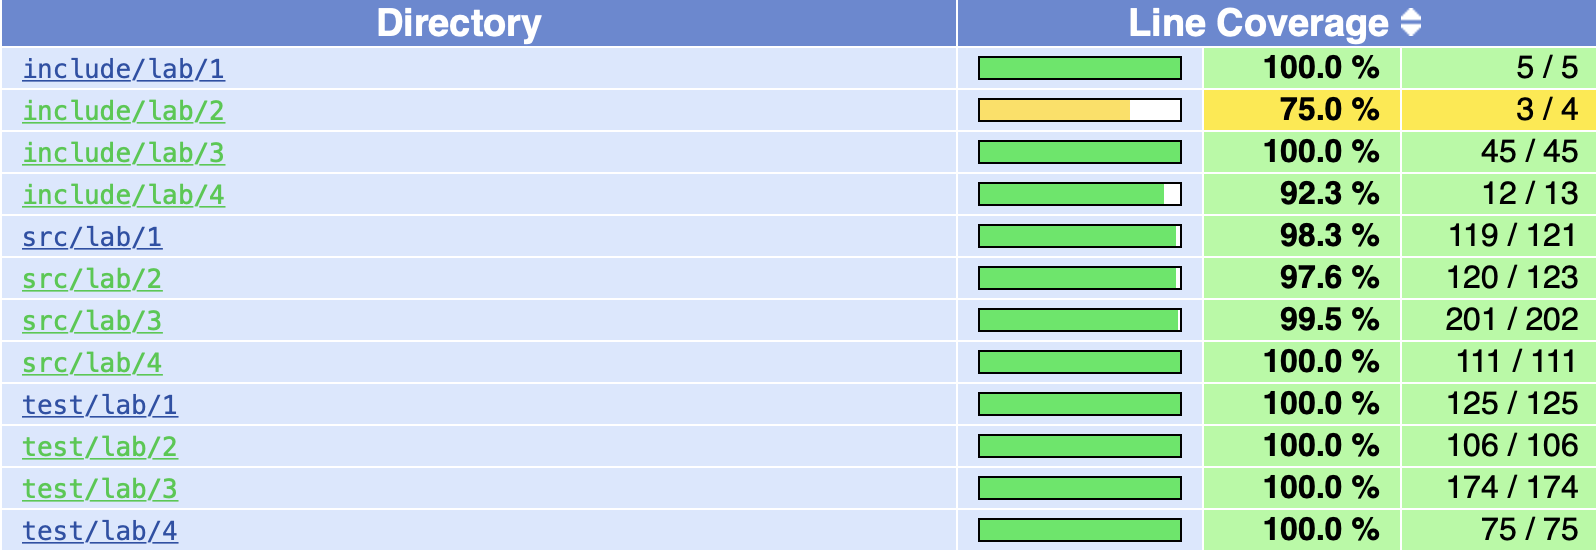
\includegraphics[scale=.5]{cov.png}
\end{figure}

\section{实验结果与分析}\label{sec:test34}
本次实验加深了对二叉树的概念、基本运算的理解,
掌握了二叉树的基本运算的实现。
深刻理解了二叉树的\emph{逻辑结构}和\emph{物理结构}之间的关系。
并通过与实验一的对比,了解到了二叉树不同的物理存储结构之间的相同点与不同点。
\par
作为第二次实验,本次实验的内容还是相对比较简单的,通过整个编程过程,我又熟悉了一遍链二叉树的实现,对原先的知识进行了一次很好的复习。
\par 整个实验均在\texttt{UNIX}环境下编程
所有的代码均采用\emph{Google C/C++}标准代码规范,
通过\texttt{clang-format}和\texttt{clang-tidy}进行格式化和规范化。
\par
同时,在编码过程中,我尽可能地使用了更加现代化的C++代码,例如使用智能指针(\textit{unique\_ptr})来进行资源管理,从而避免了手动管理内存而可能带来的内存泄漏等问题、
例如使用\texttt{auto}关键字来声明函数与变量,从而减少了错误的类型声明或不正确的隐式类型转换。
使得代码可读性更高,更容易维护,更加健壮。这样的规范和编码习惯有助于以后在工作中更高效地完成工作任务。
\par
本系统完整的实现了课程要求的全部功能,并且实现了多二叉树管理和文件存储功能,
系统健壮性良好,可以应对各种情况的输入,且能输出相应的错误提示。
系统测试覆盖度接近100\%,可以认为不会发生逻辑错误
\par

